\documentclass{beamer}
\mode <presentation>
{
    \usetheme{boxes}
    \usecolortheme{crane}
    \setbeamercovered{transparent}
}

\usepackage[absolute,overlay]{textpos}
\usepackage{pgf,pgfarrows,pgfnodes}
\usepackage[english]{babel}
\usepackage{lmodern}
\usepackage{newcent}
\usepackage{amsmath}
% math extension - one probably wants to use symbols like '[' (written as '$[$')
\usepackage{ucs}
%\usepackage[utf8]{inputenc}
%\usefonttheme{structuresmallcapsserif}

% utf8x does not work with xetex
\usepackage[utf8x]{inputenc}

\usepackage[normalem]{ulem}


\setlength{\TPHorizModule}{1mm}
\setlength{\TPVertModule}{1mm}
\newcommand{\WorkInProgress}{%
\begin{textblock}{14}(120.0,75.7)

\includegraphics[height=0.7cm]{./pics/workinprogress.jpg}
\end{textblock}
  }

%\setbeamercolor{background canvas}{bg=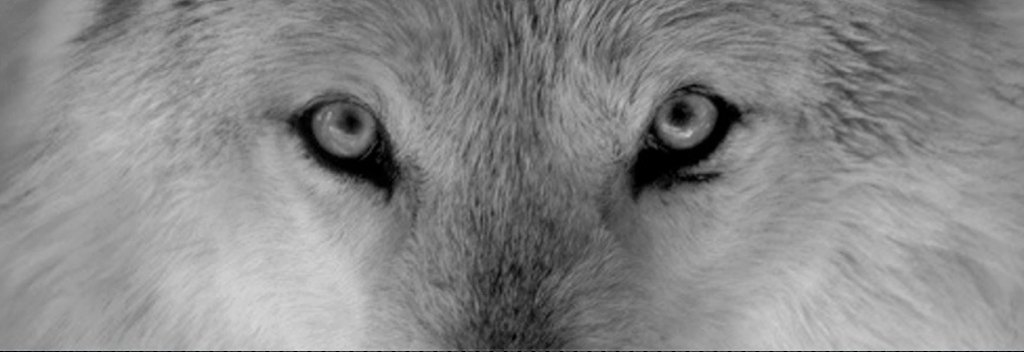
\includegraphics[width=\textwidth]{./pics/wolf.png}}

\title{Assets management with~FusionInventory~and~GLPI}
\author{\href{http://www.FusionInventory.org}{FusionInventory.org}}
\subject{Assets management with FusionInventory and GLPI}
\keywords{Assets management, Inventory, FusionInventory, GLPI}

\date{July 2011}
%\titlegraphic{GLPI}
%subtitle{
\includegraphics[width=1.2cm]{./pics/fusioninventory-logo.png}}
\institute{
\includegraphics[height=4.2cm]{./pics/rmll2011.jpg}}

\titlegraphic{}
%subtitle{
\includegraphics[width=1.2cm]{./pics/fusioninventory-logo.png}}
%\institute{
\includegraphics[height=4.2cm]{./pics/fusioninventory-logo.pdf}}
\author{ David Durieux \texttt{<d.durieux@siprossii.com>} \\
Gonéri Le Bouder \texttt{<goneri@teclib.com>}}
\logo{
\includegraphics[height=0.7cm]{./pics/fusioninventory-logo.pdf}}

\AtBeginSection[] % Do nothing for \section*
{
    \begin{frame}<beamer>
        \frametitle{Outline}
        \tableofcontents[currentsection]
    \end{frame}
}

%%%%%%%%%%%%%%%%%%%%%%%%%%%%%%%%%%%%%%%%%%%%%%%
%%%%%%%%%%%%%%%%%%%%%%%%%%%%%%%%%%%%%%%%%%%%%%%
\begin{document}

\frame[plain]{\titlepage}

\begin{frame}
    \frametitle{About us: David Durieux}

    \begin{block}{IT management consultant}
        \begin{itemize}
        \item GLPI core-developer
        \item FusionInventory project co-leader
        \item Work at siprossii, Lyon area, France
        \end{itemize}
    \end{block}

\end{frame}



\begin{frame}
    \frametitle{About us: Gonéri Le Bouder}


    \begin{block}{Free software enthusiast}
        \begin{itemize}
        \item Debian Developer
        \item Perl Monger
        \item Former OCS Inventory developer
        \item FusionInventory project co-leader
        \item Work at TECLIB', Paris, France
        \end{itemize}
    \end{block}

\end{frame}


\begin{frame}
    \frametitle{The FusionInventory contributors}

    \begin{center}
    
\includegraphics[height=3.5cm]{./pics/sparta.jpg}
    \end{center}

    \begin{itemize}
    \item about 10 developers involved in the project
    \item active community of contributors
    \item 2 companies involved
    \end{itemize}

    \pause
    \bf{We are looking for people to JOIN US!}
\end{frame}

\begin{frame}
    \frametitle{The origin}

    \begin{description}
      \item[2006] Agent creation
      \item[2008] Server project (Tracker, a GLPI plugin)
      \item[2009] Agent/Server integration 
      \item[2010] FusionInventory project
      \item[2010] Uranos integration
      \item[2011] Rudder integration
    \end{description}

\end{frame}



\begin{frame}
    \frametitle{The project infrastructure}
    %%-------------------------------------------------------------------
    %%\logo{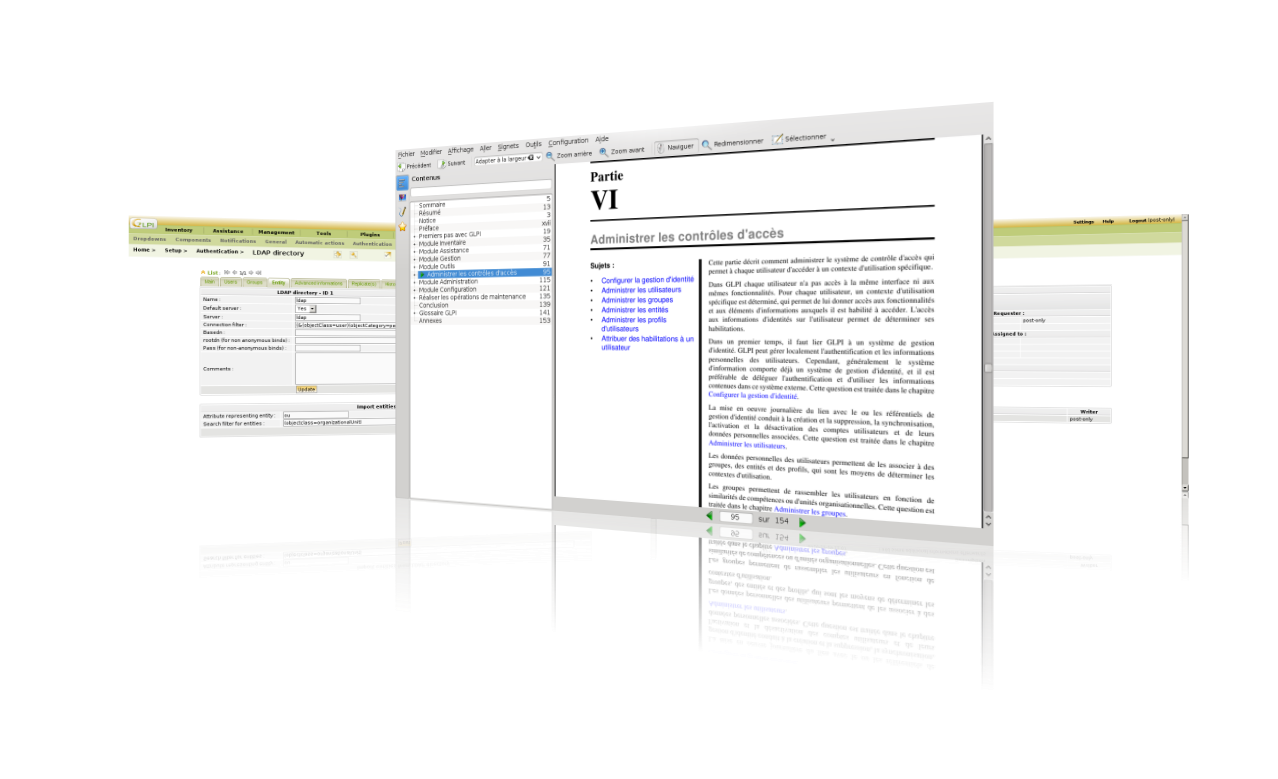
\includegraphics[height=3.5cm]{./pics/glpi-doc.png}}
    FusionInventory is a community-driven project.

    \begin{itemize}
        \item active mailing lists
        \item IRC: \#FusionInventory on FreeNode
        \item public Forge, Git repositories, etc
    \end{itemize}
\end{frame}

\section{Overview}

\begin{frame}
    \frametitle{First, some vocabulary!}

    \begin{itemize}
        \item Agent: a software running one a computer
        \item Server: a software that can speak with the Agent
        \item Task: an action done by the Agent for the server 
    \end{itemize}

\end{frame}


%%
%\begin{frame}
%    \frametitle{Agent history}
%
%    \begin{center}
%    
\includegraphics[height=3.5cm]{./pics/agent-smith.jpg}
%    \end{center}
%
%
%    \begin{itemize}
%        \item a fork of OCS Inventory UNIX agent by its author
%        \item started 5 years ago
%        \item GPLv2
%    \end{itemize}
%\end{frame}

%\begin{frame}
%    \begin{center}
%    
\includegraphics[height=4.0cm]{pics/Perl_Foundation.pdf}
%    \end{center}
%    \frametitle{use Perl Luke!}
%
%    We choose to use Perl on the agent side.
%    \begin{itemize}
%        \item portable
%        \item reliable
%        \item versatile
%        \item stable API
%    \end{itemize}
%\end{frame}

%\begin{frame}
%    \frametitle{Agent pull}
%
%    \begin{center}
%
%%    
\includegraphics[height=5.0cm]{pics/kung-fu-panda.jpg}
%
%    \end{center}
%
%\end{frame}

\begin{frame}
    \frametitle{pull / push}

    \begin{block}{FusionInventory supports "push" and "pull"}
    \begin{itemize}
    \item \textbf{"pull": Agent $\Longrightarrow$ Server} \\
    the agent creates the connection to the server.
    \item \textbf{"push": Agent $\Longleftarrow$ Server} \\
    the server awake the agent by itself.
    \end{itemize}
    \end{block}

\end{frame}

\begin{frame}
    \frametitle{Tasks}
    %
    Different Tasks are supported:
    \begin{itemize}

        \item Inventory
        \item Network discovery
        \item Remote inventory
        \item Software deployment
        \item vCenter/ESX/ESXi remote inventory
        \item Wake On Lan
    \end{itemize}
\end{frame}

\begin{frame}
    \frametitle{Servers today}

    \begin{block}{4 different servers (so far!)}
        \begin{itemize}
            \item FusionInventory for GLPI \\
            \url{http://www.FusionInventory.org}
            \item Uranos \\
            \url{http://uranos.sourceforge.net/}
            \item Rudder \\
            \url{http://www.normation.com/\#produits}
            \item OCS Inventory NG (patched to ignore the UserAgent filter) \\
            \url{http://forge.fusioninventory.org/projects/fusioninventory-agent/wiki/Patch\_ocs\_server}
        \end{itemize}
        ...local mode is also possible for Inventory
    \end{block}

\end{frame}


%\subsection{Use cases}
%\begin{frame}
    \frametitle{The inventories}

    \begin{description}
        \item[BIOS], serial numbers, UUID, etc local
        \item[Memory], memory slot, size, etc
        \item[CPU], frequency, name, manufacturer, etc
        \item[Software], apt-get, yum, Windows software, BSD pkg, etc
        \item[Harddrive], serial number, manufacturer, etc
        \item[Partition], etc
        \item[Virtual Machine], libvirt, xen, etc
        \item[USB devices], phone, USB key, etc
        \item[etc], \href{http://search.cpan.org/dist/FusionInventory-Agent/lib/FusionInventory/Agent/XML/Query/Inventory.pm}{see the list on Internet.}
    \end{description}

    It's easy to add new information. Just ask us or submit patches!

\end{frame}

\begin{frame}
    \frametitle{Identify devices on the network}

    \begin{itemize}
        \item TODO
    \end{itemize}
\end{frame}

\begin{frame}
    \frametitle{Switch inventory}

    \begin{itemize}
        \item TODO
    \end{itemize}
\end{frame}

\begin{frame}
    \frametitle{printer too!}

    \begin{itemize}
        \item TODO
    \end{itemize}
\end{frame}

\begin{frame}
    \frametitle{Wake on LAN}

    \begin{itemize}
        \item TODO
    \end{itemize}
\end{frame}

\begin{frame}
    \frametitle{Software deployment}

    \begin{itemize}
        \item TODO
    \end{itemize}
\end{frame}

\begin{frame}
    \frametitle{Task Scheduling}

    \begin{itemize}
        \item TODO
    \end{itemize}
\end{frame}

\begin{frame}
    \frametitle{libFusionInventory}
    
    \begin{itemize}
        \item TODO
    \end{itemize}
\end{frame}



\section{Installation}

\begin{frame}
    \frametitle{Server: Installation}

    \begin{block}{FusionInventory for GLPI}
        A GLPI generic plugin.
        \begin{enumerate}
            \item Extract
            \item Configure
            \item You're done!
        \end{enumerate}
    \end{block}

\end{frame}



\begin{frame}
    \frametitle{Agent: supported OS (1/2)}

    
\includegraphics[height=4.5cm]{pics/sonic.pdf}
    Runs everywhere!

    \pause

    \begin{block}{A large collection of supported OS}
        \begin{itemize}
            \item all the major system are supported
            \item portage is easy as soon as a Perl exist
        \end{itemize}
    \end{block}
\end{frame}

\begin{frame}
    \frametitle{Agent: supported OS (2/2)}
    Supported Operating Systems:

    \begin{itemize}
        \item<2-> Linux
        \item<3-> BSD
        \item<4-> AIX
        \item<5-> HP-UX
        \item<6-> Solaris
        \item<7-> Windows, all from 2000 to Seven 64bit
    \end{itemize}


    \uncover<8->{\href{http://forge.fusioninventory.org/projects/fusioninventory-agent/wiki/Agent\_supportedplateforms}{A complete list is avallable on the website}}


\includegraphics[height=0.5cm]{pics/logos/aix.png}

\includegraphics[height=0.5cm]{pics/logos/fedora.png}

\includegraphics[height=0.5cm]{pics/logos/hp-ux.png}

\includegraphics[height=0.5cm]{pics/logos/netbsd.png}

\includegraphics[height=0.5cm]{pics/logos/openbsd.png}

\includegraphics[height=0.5cm]{pics/logos/solaris.jpg}

\includegraphics[height=0.5cm]{pics/logos/centos.jpg}

\includegraphics[height=0.5cm]{pics/logos/linux.png}

\includegraphics[height=0.5cm]{pics/logos/osx.png}

\includegraphics[height=0.5cm]{pics/logos/ubuntu.png}

\includegraphics[height=0.5cm]{pics/logos/debian.png}

\includegraphics[height=0.5cm]{pics/logos/freebsd.png}

\includegraphics[height=0.5cm]{pics/logos/redhat.png}

\includegraphics[height=0.5cm]{pics/logos/windows.jpg}

\includegraphics[height=0.5cm]{pics/logos/dragonflybsd.png}

\includegraphics[height=0.5cm]{pics/logos/mageia.png}

\end{frame}


\begin{frame}
    \frametitle{Agent: Tested systems}

    \begin{block}{Linux}
        \begin{itemize}
            \item \textbf{Debian} all since 3.1
            \item \textbf{Ubuntu} all since 8.04
            \item \textbf{Mandriva} 2007.1, 2010.0, 2010.1
            \item \textbf{MandrakeLinux} 9.2, 10.2
            \item \textbf{Slackware} 10 to 13
            \item \textbf{Fedora} all since the 2nd
            \item \textbf{RedHat Linux} 7.0, 8.0 and 9.0
            \item \textbf{RedHat Enterprise Linux} (or CentOS) all since 3
            \item \textbf{SME Server} 7.5
            \item \textbf{OpenSUSE} 11.3
            \item \textbf{Gentoo} 1.6.14, 2008
            \item \textbf{Montavista} 4.0 
            \item \textbf{SUSE Linux Enterprise Server} 10, 11 
        \end{itemize}
    \end{block}
\end{frame}

\begin{frame}
    \frametitle{Agent: Tested systems}

    \begin{block}{Windows}
        \begin{itemize}
            \item \textbf{Windows 2000} $\geq$ SP4
            \item \textbf{Windows XP} all
            \item \textbf{Windows 2003} all
            \item \textbf{Windows 2008} all
            \item \textbf{Windows Vista} all
            \item \textbf{Windows Seven} all
        \end{itemize}
    \end{block}
\end{frame}

\begin{frame}
    \frametitle{Agent: Tested systems}

    \begin{block}{MacOSX}
        \begin{itemize}
            \item \textbf{Panther} 10.3.9 PowerPC
            \item \textbf{Tiger} all 
            \item \textbf{Leopard} all
            \item \textbf{Snow Leopard} all
        \end{itemize}
    \end{block}
\end{frame}

\begin{frame}
    \frametitle{Agent: Tested systems}

    \begin{block}{Solaris}
        \begin{itemize}
            \item \textbf{Solaris} 8 to 10 for SPARC and 10 to 11 for x86
            \item \textbf{OpenSolaris} 2009.06
            \item \textbf{OpenIndiana} oi\_148
        \end{itemize}
    \end{block}
\end{frame}

\begin{frame}
    \frametitle{Agent: Tested systems}

    \begin{block}{BSD}
        \begin{itemize}
            \item \textbf{OpenBSD} 4.5 to 4.8
            \item \textbf{FreeBSD} all since 5.3 include Debian GNU/kFreeBSD
            \item \textbf{NetBSD} 5.0 and 5.1
            \item \textbf{DragonflyBSD} 2.8
        \end{itemize}
    \end{block}
\end{frame}


\begin{frame}
    \frametitle{Agent: Tested systems}

    \begin{block}{HPUX}
        \begin{itemize}
            \item \textbf{11.11} PA-RISC
            \item \textbf{11.23} Itanium
            \item \textbf{11.31} Itanium
        \end{itemize}
    \end{block}
\end{frame}

\begin{frame}
    \frametitle{Agent: Tested systems}

    \begin{block}{AIX}
        \begin{itemize}
            \item \textbf{5.1}
            \item \textbf{5.2}
            \item \textbf{6.1}
        \end{itemize}
    \end{block}
\end{frame}



\begin{frame}
    \frametitle{Agent: Installation}


    \begin{block}{different options}
        \begin{itemize}
            \item distribution packages \\
            \small{Debian, Fedora, EPEL, Ubuntu, Mageia, ...}
            \item Windows installer \\
            \small{GPO, psexec, ...}
            \item static prebuilt packages, untar and run \\
            \small{53 differents system so far}
            \item tarball or CPAN installation
        \end{itemize}
    \end{block}
\end{frame}




\section{Inventory}

\begin{frame}

    \frametitle{The inventory content}

This section presents the XML structure used by FusionInventory.

%    \begin{description}
%        \item[BIOS] serial numbers, UUID, ... local
%        \item[Memory] memory slot, size, ...
%        \item[CPU] frequency, name, manufacturer, ...
%        \item[Software] apt-get, yum, Windows software, BSD pkg, ...
%        \item[Harddrive] serial number, manufacturer, ...
%        \item[Partition] ...
%        \item[Virtual Machine] libvirt, xen, ...
%        \item[USB devices] phone, USB key, ...
%        \item[...] \href{http://search.cpan.org/dist/FusionInventory-Agent/lib/FusionInventory/Agent/XML/Query/Inventory.pm}{see the list on Internet.}
%    \end{description}

%    It's easy to add new information. Just ask us or submit patches!

\end{frame}

\begin{frame}
\frametitle{Inventory: Generic machine information (1/3)}
\begin{description}
      \item[USERID] The current user list, '/' is the delimiter. This field is deprecated, you should use the USERS section instead.
      \item[OSVERSION]
      \item[OSCOMMENTS] Service Pack on Windows, kernel build date on Linux
      \item[CHECKSUM] Deprecated, OCS only.
      \item[PROCESSORT] Deprecated, OCS only.
      \item[NAME]
      \item[PROCESSORS] The processor speed in MHz, this field is deprecated, see CPUS instead.
      \item[SWAP] The swap space in MB.
\end{description}
\end{frame}
\begin{frame}
\frametitle{Inventory: Generic machine information (2/3)}
\begin{description}

      \item[ETIME] The time needed to run the inventory on the agent side.
      \item[OSNAME]
      \item[IPADDR]
      \item[WORKGROUP]
      \item[DESCRIPTION] Computer description (Windows only so far)
      \item[MEMORY] Total system memory in MB
      \item[UUID]
      \item[DNS]
      \item[LASTLOGGEDUSER] The login of the last logged user.
      \item[USERDOMAIN] This field is deprecated, you should use the USERS section instead.
      \item[DATELASTLOGGEDUSER]
\end{description}
\end{frame}
\begin{frame}
\frametitle{Inventory: Generic machine information  (3/3)}
\begin{description}
      \item[DEFAULTGATEWAY]
      \item[VMSYSTEM] The virtualization technologie used if the machine is a virtual machine.
 Can by:
 Physical: (default) Xen VirtualBox Virtual Machine: Generic if it's not possible to correctly identify the solution VMware: ESX, ESXi, server, etc QEMU SolarisZone VServer OpenVZ BSDJail Parallels Hyper-V
      \item[WINOWNER]
      \item[WINPRODID]
      \item[WINPRODKEY]
      \item[WINCOMPANY] 
      \item[WINLANG] Language code of the Windows
      \item[CHASSIS\_TYPE] The computer chassis format (e.g: Notebook, Laptop, Server, etc)
\end{description}
\end{frame}

\begin{frame}
\frametitle{Inventory: BIOS}
\begin{description}
      \item[SMODEL] System model
      \item[SMANUFACTURER] System manufacturer
      \item[SSN] System Serial number
      \item[BDATE] BIOS release date
      \item[BVERSION] The BIOS revision
      \item[BMANUFACTURER] BIOS manufacturer
      \item[MMANUFACTURER] Motherboard Manufacturer
      \item[MSN Motherboard Serial]
      \item[MMODEL] Motherboard model
      \item[ASSETTAG]
      \item[ENCLOSURESERIAL]
      \item[BASEBOARDSERIAL]
      \item[BIOSSERIAL] The optional asset tag for this machine.
\end{description}

\end{frame}
\begin{frame}

\frametitle{Inventory: PCI cards}
\begin{description}
      \item[DRIVER]
      \item[NAME] The device name, the on from the PCIIDs DB
      \item[MANUFACTURER] The manifacturer name, the on from the PCIIDs DB
      \item[PCICLASS] The PCI class ID
      \item[PCIID] The PCI ID, e.g: 8086:2a40 (only for PCI device)
      \item[PCISUBSYSTEMID] The PCI subsystem ID, e.g: 8086:2a40 (only for PCI device)
      \item[PCISLOT] The PCI slot, e.g: 00:02.1 (only for PCI device)
      \item[TYPE] The controller revision, e.g: rev 02. This field may be renamed in the future.
      \item[REV] Revision of the device in the XX format (e.g: 04)
\end{description}
\end{frame}

\begin{frame}
\frametitle{Inventory: Memories}
\begin{description}
      \item[DESCRIPTION]
      \item[FORMFACTOR] Only available on Windows, See Win32\_PhysicalMemory documentation on MSDN.
      \item[PURPOSE] Only avalaible on Windows, See Win32\_PhysicalMemory documentation on MSDN.
      \item[SPEED] In Mhz, e.g: 800
      \item[TYPE]
      \item[NUMSLOTS] Eg. 2, start at 1, not 0
      \item[SERIALNUMBER]
\end{description}
\end{frame}
\begin{frame}
\frametitle{Inventory: CPUs}
\begin{description}
      \item[CACHESIZE] The total CPU cache size in KB. e.g: 3072
      \item[CORE] Number of core.
      \item[DESCRIPTION]
      \item[MANUFACTURER] AMD/Intel/Transmeta/Cyrix/VIA
      \item[NAME] The name of the CPU, e.g: Intel(R) Core(TM)2 Duo CPU P8600 @ 2.40GHz
      \item[THREAD] Number of thread per core.
      \item[SERIAL] Serial number
      \item[SPEED] Frequency in MHz
      \item[ID] The CPU ID: \url{http://en.wikipedia.org/wiki/CPUID}
\end{description}
\end{frame}
\begin{frame}
\frametitle{Inventory: Filesystems}
\begin{description}
      \item[CREATEDATE] Date of creation of the filesystem in DD/MM/YYYY format.
      \item[DESCRIPTION]
      \item[FREE] Free space (MB)
      \item[FILESYSTEM] File system name. e.g: ext3
      \item[LABEL] Name of the partition given by the user.
      \item[LETTER] Windows driver letter. Windows only
      \item[SERIAL] Partition serial number or UUID
      \item[SYSTEMDRIVE] Boolean. Is this the system partition?
      \item[TOTAL] Total space available (MB)
      \item[TYPE] The mount point on UNIX.
      \item[VOLUMN] System name of the partition (e.g: /dev/sda1 or server:/directory for NFS)
\end{description}
\end{frame}
\begin{frame}
\frametitle{Inventory: Screens}
\begin{description}
      \item[BASE64] The uuencoded EDID trame. Optional.
      \item[DESCRIPTION]
      \item[MANUFACTURER] The manufacturer retrieved from the EDID trame.
      \item[SERIAL] The serial number retrieved from the EDID trame.
      \item[UUENCODE] The uuencoded EDID trame. Optional.
\end{description}
\end{frame}
\begin{frame}
\frametitle{Inventory: Storage devices}
\begin{description}
      \item[DESCRIPTION] The long name of the device displayed to the user.
      \item[DISKSIZE] The disk size in MB.
      \item[INTERFACE] INTERFACE can be SCSI/HDC/IDE/USB/1394/Serial-ATA/SAS or empty if unknown
      \item[MANUFACTURER]
      \item[MODEL] The commercial name of the device
      \item[NAME] The name of the device as seen by the system.% E.g: hda (Linux), \backslash \backslash.\backslash PHYSICALDRIVE0 (Windows)
      \item[TYPE] The kind of device. There is no standard for the format of the string in this field.
      \item[SERIAL] The harddrive serial number
      \item[FIRMWARE] Firmware version
      \item[SCSI] COID, CHID, UNID and LUN
      \item[WWN] World Wide Name \url{http://fr.wikipedia.org/wiki/World\_Wide\_Name}
\end{description}

\end{frame}
\begin{frame}
\frametitle{Inventory: Softwares}
\begin{description}
      \item[NAME]
      \item[COMMENTS]
      \item[FILESIZE]
      \item[PUBLISHER]
      \item[FOLDER]
      \item[FROM] Where the information about the software came from, can be: registry, rpm, deb, etc
      \item[INSTALLDATE] Installation day in DD/MM/YYYY format. Windows only.
      \item[NO\_REMOVE] Can the software be removed.
      \item[RELEASE\_TYPE] Windows only for now, come from the registry
      \item[UNINSTALL\_STRING] Windows only, come from the registry
      \item[URL\_INFO\_ABOUT]
      \item[VERSION]
      \item[IS64BIT] If the software is in 32 or 64bit, (1/0)
      \item[GUID] Windows software GUID
\end{description}
\end{frame}
\begin{frame}
\frametitle{Inventory: Logged users}
\begin{description}
      \item[LOGIN]
      \item[DOMAIN] The Windows domain of the user, if available.
\end{description}
\end{frame}
\begin{frame}
\frametitle{Inventory: Video cards}
\begin{description}
      \item[CHIPSET]
      \item[MEMORY] Video card memory in MB
      \item[NAME]
      \item[RESOLUTION] Resolution in pixel. 1024x768.
      \item[PCISLOT] The local PCI slot ID if the video card use PCI.
\end{description}
\end{frame}
\begin{frame}
\frametitle{Inventory: Virtual machines}
\begin{description}
      \item[MEMORY] Memory size, in MB.
      \item[NAME] The name of the virtual machine.
      \item[UUID]
      \item[STATUS] The VM status: running, idle, paused, shutdown, crashed, dying, off
      \item[SUBSYSTEM] The virtualisation software. E.g: VmWare ESX
      \item[VMTYPE] The name of the virtualisation system family. The same type found is HARDWARE/VMSYSTEM
      \item[VCPU] Number of CPU affected to the virtual machine
      \item[VMID] The ID of virtual machine in the virtual managment system.
      \item[MAC The list of the MAC addresses of the virtual machine. The delimiter] is '/'. e.g: 00:23:18:91:db:8d/00:23:57:31:sb:8e
      \item[COMMENT] a comment
      \item[OWNER]
\end{description}
\end{frame}
\begin{frame}
\frametitle{Inventory: USB devices}
\begin{description}
      \item[VENDORID] Vendor USB ID. 4 hexa char.
      \item[PRODUCTID] Product USB ID. 4 hexa char.
      \item[SERIAL]
      \item[CLASS] USB Class (e.g: 8 for Mass Storage)
      \item[SUBCLASS] USB Sub Class
      \item[NAME] The name of the device (optional)
\end{description}
\end{frame}
\begin{frame}
\frametitle{Inventory: Network configuration (1/2)}
\begin{description}
      \item[A network configuration.]
      \item[DESCRIPTION] The name of the interface as seen in the OS settings, e.g: eth0 (Linux) or AMD PCNET Family Ethernet Adapter (Windows)
      \item[DRIVER] The name of the driver used by the network interface
      \item[IPADDRESS]
      \item[IPDHCP] The IP address of the DHCP server (optional).
      \item[IPGATEWAY]
      \item[IPMASK]
      \item[IPSUBNET]
\end{description}
\end{frame}
\begin{frame}
\frametitle{Inventory: Network configuration (2/2)}
\begin{description}
      \item[MACADDR]
      \item[MTU]
      \item[PCISLOT] The PCI slot name.
      \item[STATUS] Up or Down
      \item[TYPE] Interface type: Ethernet, Wifi
      \item[VIRTUALDEV] If the interface exist or not (1 or empty)
      \item[SLAVES] Bonded interfaces list in the eth0/eth1/eth2 format (/ is the separator).
      \item[MANAGEMENT] Whether or not it is a HP iLO, Sun SC, HP MP or other kind of Remote Management Interface
      \item[SPEED] Interface speed in Mb/s
      \item[BSSID] Wifi only, Access point MAC Address
      \item[SSID] Wifi only, Access point name
\end{description}
\end{frame}
\begin{frame}
\frametitle{Inventory: Batteries (laptop computer)}
\begin{description}
      \item[CAPACITY] Battery capacity in mWh
      \item[DATE] Manufacture date in DD/MM/YYYY format
      \item[NAME] Name of the device
      \item[SERIAL] Serial number
      \item[MANUFACTURER] Battery manufacturer
      \item[VOLTAGE] Voltage in mV
\end{description}
\end{frame}
\begin{frame}
\frametitle{Inventory: Printers}
\begin{description}
      \item[COMMENT]
      \item[DESCRIPTION]
      \item[DRIVER]
      \item[NAME]
      \item[NETWORK] Network: True (1) if it's a network printer
      \item[PORT]
      \item[RESOLUTION] Resolution: eg. 600x600
      \item[SHARED] Shared: True if the printer is shared (Win32)
      \item[STATUS] Status: See Win32\_Printer.PrinterStatus
      \item[ERRSTATUS] ErrStatus: See Win32\_Printer.ExtendedDetectedErrorState
      \item[SERVERNAME]
      \item[SHARENAME]
      \item[SERIAL] The serial number
\end{description}
\end{frame}
\begin{frame}
\frametitle{Inventory: Running processes}
\begin{description}
      \item[USER] The process owner
      \item[PID The process Id]
      \item[CPUUSAGE] The CPU usage.
      \item[MEM The memory.]
      \item[VIRTUALMEMORY]
      \item[TTY]
      \item[STARTED] When the process has been started in YYYY/MM/DD HH:MM format
      \item[CMD The command.]
\end{description}
\end{frame}
\begin{frame}
\frametitle{Inventory: AntiVirus software}
\begin{description}
      \item[COMPANY] Comapny name
      \item[NAME]
      \item[GUID] Unique ID
      \item[ENABLED] 1 if the antivirus is enabled.
      \item[UPTODATE] 1 if the antivirus is up to date.
      \item[VERSION]
\end{description}
\end{frame}
\begin{frame}
\frametitle{Inventory: LVM Logical Volumes}
\begin{description}
      \item[LVNAME] The volume name.
      \item[VGNAME] The volume group name.
      \item[ATTR] The special attribue used on this volume (e.g: a-)
      \item[SIZE] The size of the volume on MB.
      \item[UUID] The volume UUID.
\end{description}
\end{frame}
\begin{frame}
\frametitle{Inventory: LVM Physical volumes}
\begin{description}
      \item[DEVICE] The device name. Eg.: /dev/sda1 on Linux.
      \item[PV\_NAME] The physical device name.
      \item[FORMAT] The format. E.g: lvm2.
      \item[ATTR] The LVM attribue in use for this phyisical device.
      \item[SIZE] The size in MB.
      \item[PV\_UUID] The UUID.
      \item[PV\_PE\_COUNT] Item PV\_PE\_COUNT
      \item[PE\_SIZE] Item PE\_SIZE
\end{description}
\end{frame}
\begin{frame}
\frametitle{Inventory: LVM Volume group}
\begin{description}
      \item[VGNAME] The name of the volume group.
      \item[PV\_COUNT]
      \item[LV\_COUNT]
      \item[ATTR] The volume group LVM attribue.
      \item[SIZE] The size.
      \item[FREE] The free space.
      \item[UUID] The UUID
\end{description}
\end{frame}
\begin{frame}
\frametitle{Inventory: Environment variables}
\begin{description}
      \item[KEY] The variable name
      \item[VAL] The content
\end{description}
\end{frame}


\begin{frame}
\frametitle{Inventory: Ports}
\begin{description}
      \item[Serial, Parallel, SATA, etc]
      \item[DESCRIPTION]
      \item[NAME]
      \item[TYPE]
\end{description}
\end{frame}

\begin{frame}
\frametitle{Inventory: Slots}
\begin{description}
      \item[CAPACITY]
      \item[FORMFACTOR]
      \item[REMOVABLE]
      \item[TYPE]
      \item[DESCRIPTION]
\end{description}
\end{frame}
\begin{frame}
\frametitle{Inventory: Sound cards}
\begin{description}
      \item[DESCRIPTION]
      \item[MANUFACTURER]
      \item[NAME]
\end{description}
\end{frame}
\begin{frame}
\frametitle{Inventory: Modems}
\begin{description}
      \item[DESCRIPTION]
      \item[NAME]
\end{description}
\end{frame}

\section{Network Discovery}

\begin{frame}
    \frametitle{Network discovery}

    FusionInventory can do basic network inventory in GLPI
    \begin{block}{Seek}
    \begin{itemize}
      \item nmap
      \item netbios
      \item SNMP query
    \end{itemize}
    \end{block}
    \begin{block}{Identify}
    \begin{itemize}
        \item network stack
        \item Windows domain information
        \item sysdesc comparaison
    \end{itemize}
    \end{block}
\end{frame}

\section{SNMP}
\begin{frame}
    \frametitle{Remote SNMP inventory}

    \begin{block}{Network devices}
        \begin{itemize}
            \item serial number, firmware, ...
            \item ports mapping
        \end{itemize}
    \end{block}

    \begin{block}{Network printers}
        \begin{itemize}
            \item serial number, firmware, ...
            \item cartridge ink level
            \item page counter
        \end{itemize}
    \end{block}
\end{frame}




\begin{frame}
    \frametitle{SNMP: Goal}

    \begin{itemize}
    \item Identify devices remotly
    \item Inventory devices by SNMP
    \end{itemize}
\end{frame}

\begin{frame}
    \frametitle{SNMP: history}

    \begin{itemize}
    \item Created in 1992
    \item Created for monitoring devices
    \item Some RFC are writen to implement it with standard
    \end{itemize}
\end{frame}

\begin{frame}
    \frametitle{SNMP: Why create own models}

    MIB exists but
    \begin{itemize}
    \item Difficult to find (not for all of course)
    \item MIB not complete
    \item OID not always same on device (depend of model and firmware)
    \end{itemize}
    With models, we are sure device is very nice supported!
\end{frame}

\begin{frame}
    \frametitle{SNMP: What is these models}

    We store these informations
    \begin{itemize}
    \item Relation OID with information (like serial number is oid .1.3...)
    \item Simple or dynamic OID (a serial number or name of each port)
    \end{itemize}

    How to make them?
    \begin{itemize}
    \item We use a complete snmpwalk of each device + model + firmware
    \item Our tool permit to preselect and select OID 
    \item This tool will create and export models 
    \end{itemize}
\end{frame}

\begin{frame}
    \frametitle{SNMP: Switch specification (1/3)}

    Get switch informations 
    \begin{itemize}
    \item Serial number
    \item Manufacturer
    \item Model
    \item Firmware
    \item Mac address    
    \item etc
    \end{itemize}
\end{frame}

\begin{frame}
    \frametitle{SNMP: Switch specification (2/3)}

    Get ports
    \begin{itemize}
    \item Name
    \item Network speed
    \item Port status (enabled / disabled)
    \item Errors input \& output
    \item VLAN
    \item Trunk (tagged)
    \item Active connection
    \end{itemize}
\end{frame}

\begin{frame}
    \frametitle{SNMP: Switch specification (3/3)}

    Get connections on each port
    \begin{itemize}
    \item Mac addresses (one or many on some case)
    \item LLDP \& CDP neighbors (dialog \& informations  between switches)
    \end{itemize}
\end{frame}

\section{Software Deployment}

\begin{frame}
    \frametitle{Software Deployment: OCS Inventory}

    \begin{block}{What?}
    OCS software deployment support featuring peer to peer support
    \end{block}

    \begin{block}{Benefit}
    \begin{itemize}
        \item no proxy nor mirror
        \item bandwidth-friendly
        \item OS independent
    \end{itemize}
    \end{block}
\end{frame}


\begin{frame}
    \frametitle{Software Deployment: FusionInventory}

    \begin{block}{What?}
    FusionInventory deployment support featuring peer to peer support
    \end{block}

    \begin{block}{Benefit}
    \begin{itemize}
        \item no proxy nor mirror
        \item bandwidth-friendly
        \item OS independent
    \end{itemize}
    \end{block}

\WorkInProgress
\end{frame}


\section{vCenter/ESX/ESXi remote inventory}

\section{Wake On Line}

\begin{frame}
    \frametitle{Wake on LAN}

    \begin{block}{What?}
    \begin{itemize}
        \item awake computer.
    \end{itemize}
    \end{block}

\pause

    \begin{block}{How?}
    send the Magic Packet from an agent in the same network
    \begin{itemize}
        \item send raw ethernet packet
        \item UDP packet still possible
    \end{itemize}
    \end{block}

\pause

    \begin{block}{Benefit}
    \begin{itemize}
        \item no firewall issue
        \item nor special routage rule needed
    \end{itemize}
    \end{block}

\end{frame}


\section{What else?}


\begin{frame}
    \frametitle{What else? (1/2)}

    \begin{center}
    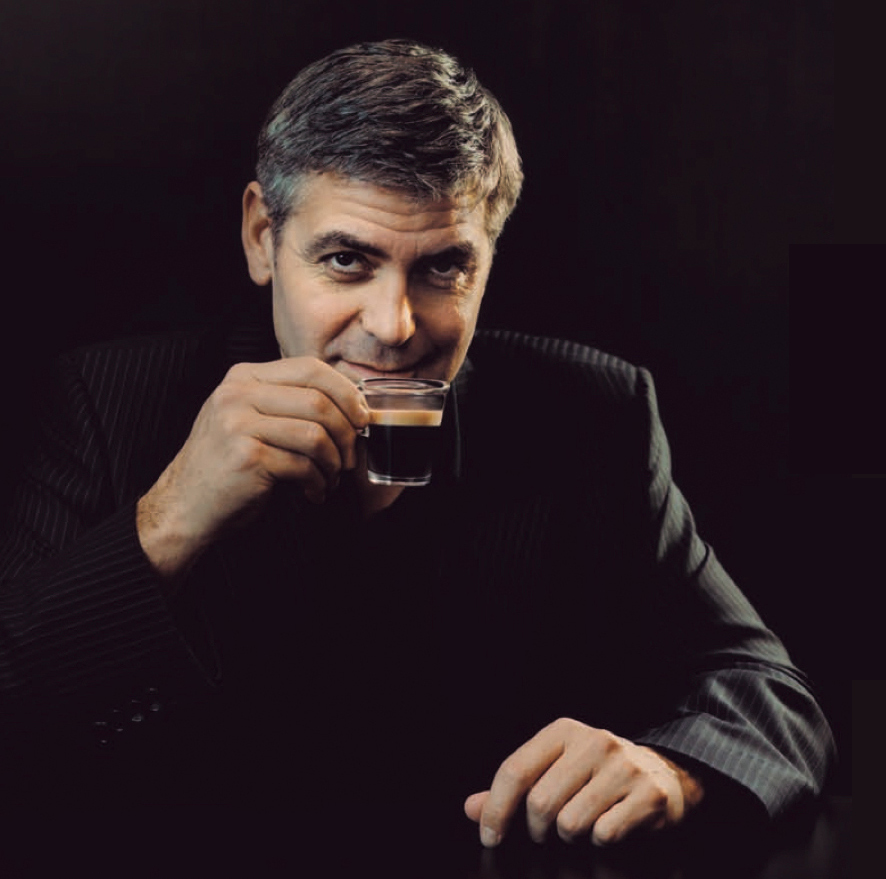
\includegraphics[height=4.0cm]{pics/whatelse.jpg}
    \end{center}

    \pause

    \begin{block}{agent developement is very active}
        \begin{itemize}
            \item code clean up\\
            {\small larger test-suite, modern perl}
            \item architecture changes\\
            {\small event-driven programming, various executable}
            \item smaller memory footprint
        \end{itemize}
    \end{block}
\end{frame}

\begin{frame}
    \frametitle{What else? (2/2)}

    \begin{center}
    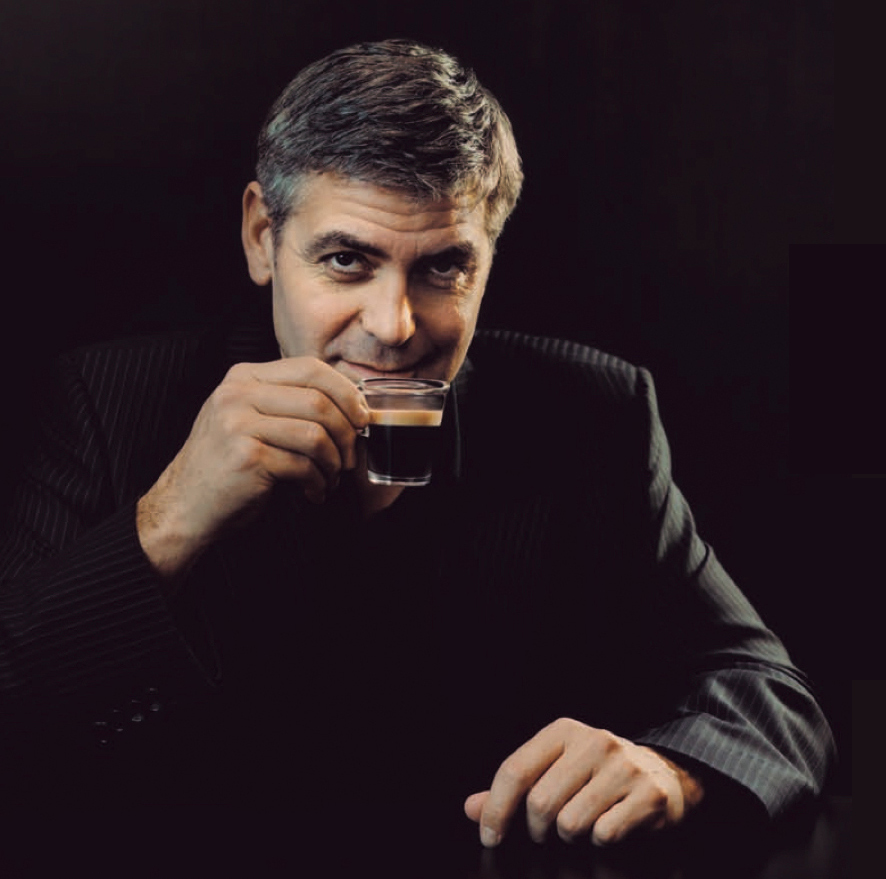
\includegraphics[height=4.0cm]{pics/whatelse.jpg}
    \end{center}

    \begin{block}{In test-suite we trust!}
        \begin{itemize}
            \item strong effort done during the last year \\
            \small{36 800 tests on the GLPI plugin and up to 2 000 on the agent}
            \item with even stronger benefit so far
        \end{itemize}
    \end{block}
\end{frame}

\begin{frame}
    \frametitle{Our roadmap}

    What we are about to release
    \begin{itemize}
    \item FusionInventory for GLPI 0.78: beta planned for this month
    \item ESX inventory: before june
    \item Android Agent
    \end{itemize}

    Work in progress
    \begin{itemize}
    \item Software deployment
    \item OCS/XML → REST/JSON transition
    \end{itemize}
\end{frame}

\begin{frame}
\frametitle{FusionInventory for GLPI 0.78: Action scheduler 1/2}
    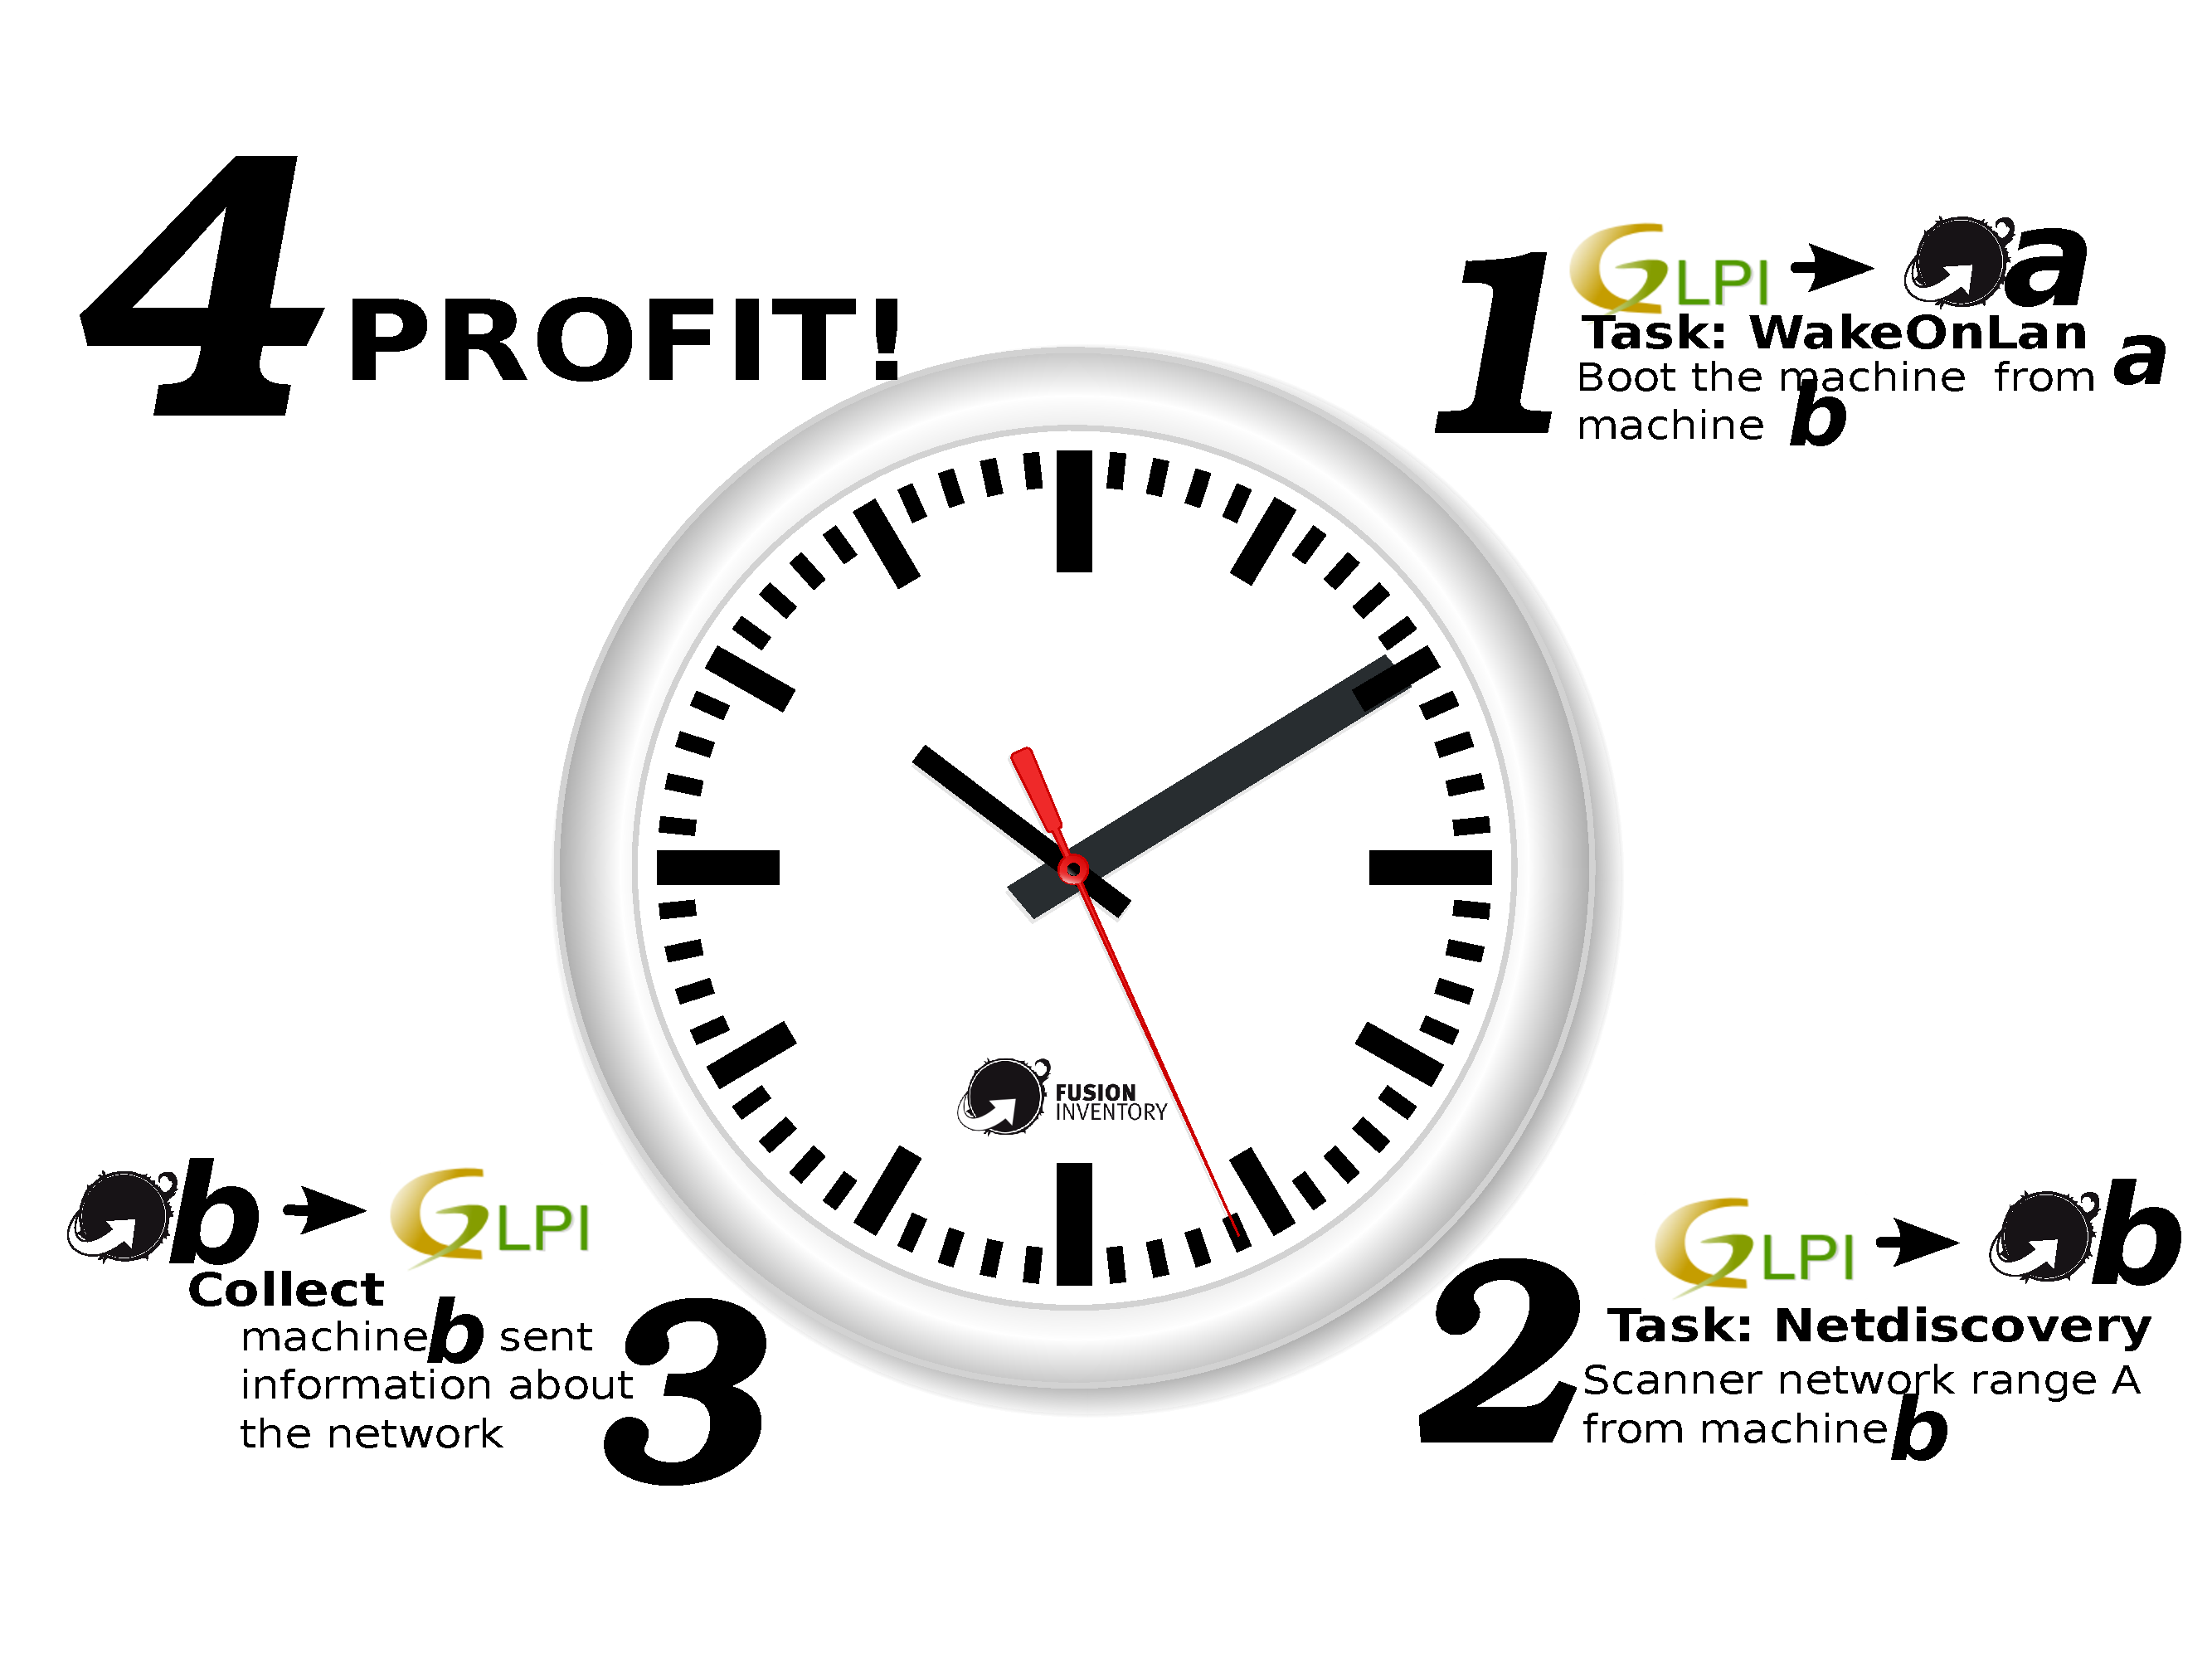
\includegraphics[height=7.5cm]{pics/fusion_task.pdf}
\end{frame}

\begin{frame}
\frametitle{FusionInventory for GLPI 0.78: Action scheduler 2/2}
    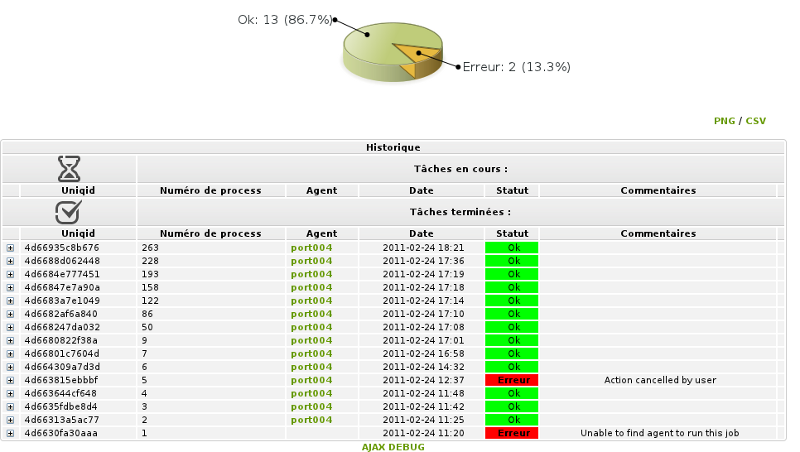
\includegraphics[height=7.5cm]{pics/walid_task_1.png}
\end{frame}

\begin{frame}
\frametitle{FusionInventory for GLPI 0.78: Printer graph}
    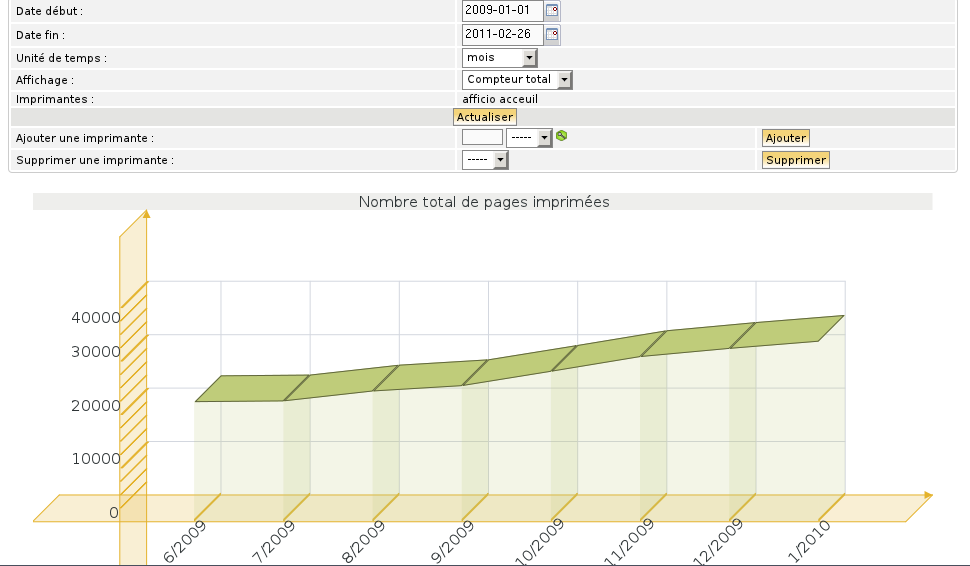
\includegraphics[height=7.5cm]{pics/walid_printer_2.png}
\end{frame}
%



\begin{frame}
\frametitle{ESX 1/2}


   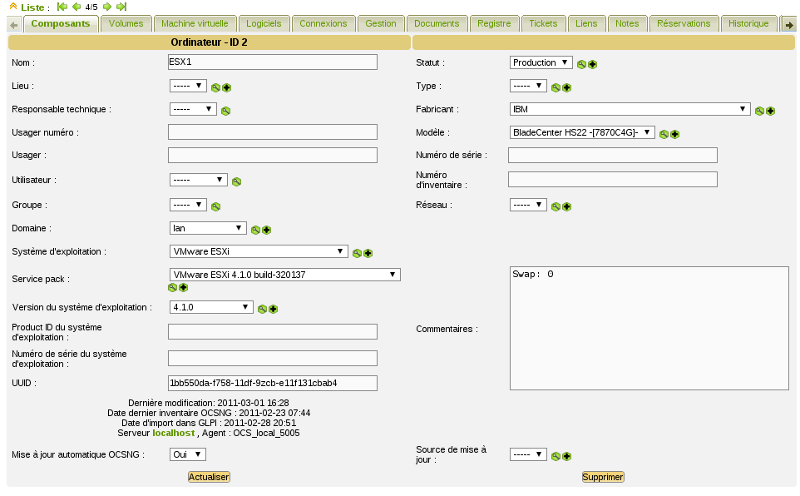
\includegraphics[height=5cm]{./pics/esx1.png}
\end{frame}
%
\begin{frame}
\frametitle{ESX 2/2}


   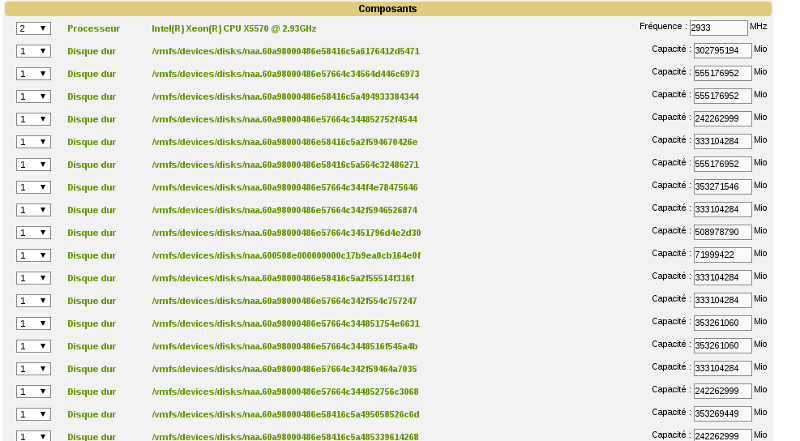
\includegraphics[height=5cm]{./pics/esx2.png}
\end{frame}

%\begin{frame}
%\frametitle{OCS/XML → REST/JSON transition}
%
%\begin{block}{Why}
%    \begin{itemize}
%    \item non standard protocol
%    \begin{itemize}
%    \item unhard to extend: parameters send once whatever you do
%    \item odd XML structure to parse
%    \item hard to extend
%    \end{itemize}
%    \item more modern alternative nowaday
%    \begin{itemize}
%    \item REST
%    \item JSON
%    \end{itemize}
%    \end{itemize}
%\end{block}
%
% \begin{block}{How this will be achieved}
%    \begin{itemize}
%    \item Long transition with dual system
%    \item keep OCS inventory compatibiliy
%    \end{itemize}
%\end{block}

%\end{frame}

\begin{frame}
    \frametitle{Demo}

   
\includegraphics[height=5cm]{./pics/fusinvglpi.png}

    \bf{Demo time!}
\end{frame}


\section{Questions}

\begin{frame}
    \frametitle{Questions?}

%    \bf{Questions?}
    \begin{center}

    
\includegraphics[height=5cm]{./pics/question.pdf}

    \end{center}
%    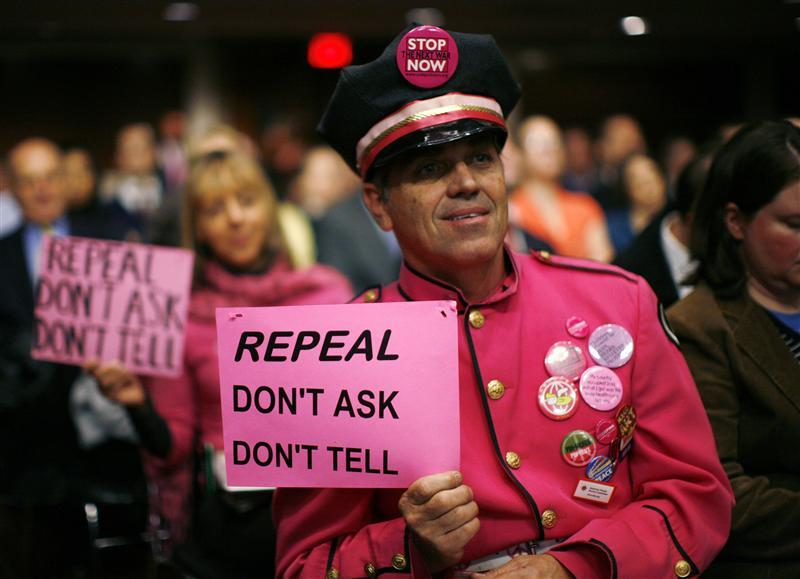
\includegraphics[height=7.5cm]{./pics/ask.jpg}

\end{frame}



\end{document}
